% Options for packages loaded elsewhere
\PassOptionsToPackage{unicode}{hyperref}
\PassOptionsToPackage{hyphens}{url}
%
\documentclass[
  ,man]{apa7}
\usepackage{amsmath,amssymb}
\usepackage{iftex}
\ifPDFTeX
  \usepackage[T1]{fontenc}
  \usepackage[utf8]{inputenc}
  \usepackage{textcomp} % provide euro and other symbols
\else % if luatex or xetex
  \usepackage{unicode-math} % this also loads fontspec
  \defaultfontfeatures{Scale=MatchLowercase}
  \defaultfontfeatures[\rmfamily]{Ligatures=TeX,Scale=1}
\fi
\usepackage{lmodern}
\ifPDFTeX\else
  % xetex/luatex font selection
\fi
% Use upquote if available, for straight quotes in verbatim environments
\IfFileExists{upquote.sty}{\usepackage{upquote}}{}
\IfFileExists{microtype.sty}{% use microtype if available
  \usepackage[]{microtype}
  \UseMicrotypeSet[protrusion]{basicmath} % disable protrusion for tt fonts
}{}
\makeatletter
\@ifundefined{KOMAClassName}{% if non-KOMA class
  \IfFileExists{parskip.sty}{%
    \usepackage{parskip}
  }{% else
    \setlength{\parindent}{0pt}
    \setlength{\parskip}{6pt plus 2pt minus 1pt}}
}{% if KOMA class
  \KOMAoptions{parskip=half}}
\makeatother
\usepackage{xcolor}
\usepackage{graphicx}
\makeatletter
\def\maxwidth{\ifdim\Gin@nat@width>\linewidth\linewidth\else\Gin@nat@width\fi}
\def\maxheight{\ifdim\Gin@nat@height>\textheight\textheight\else\Gin@nat@height\fi}
\makeatother
% Scale images if necessary, so that they will not overflow the page
% margins by default, and it is still possible to overwrite the defaults
% using explicit options in \includegraphics[width, height, ...]{}
\setkeys{Gin}{width=\maxwidth,height=\maxheight,keepaspectratio}
% Set default figure placement to htbp
\makeatletter
\def\fps@figure{htbp}
\makeatother
\setlength{\emergencystretch}{3em} % prevent overfull lines
\providecommand{\tightlist}{%
  \setlength{\itemsep}{0pt}\setlength{\parskip}{0pt}}
\setcounter{secnumdepth}{-\maxdimen} % remove section numbering
% Make \paragraph and \subparagraph free-standing
\ifx\paragraph\undefined\else
  \let\oldparagraph\paragraph
  \renewcommand{\paragraph}[1]{\oldparagraph{#1}\mbox{}}
\fi
\ifx\subparagraph\undefined\else
  \let\oldsubparagraph\subparagraph
  \renewcommand{\subparagraph}[1]{\oldsubparagraph{#1}\mbox{}}
\fi
\newlength{\cslhangindent}
\setlength{\cslhangindent}{1.5em}
\newlength{\csllabelwidth}
\setlength{\csllabelwidth}{3em}
\newlength{\cslentryspacingunit} % times entry-spacing
\setlength{\cslentryspacingunit}{\parskip}
\newenvironment{CSLReferences}[2] % #1 hanging-ident, #2 entry spacing
 {% don't indent paragraphs
  \setlength{\parindent}{0pt}
  % turn on hanging indent if param 1 is 1
  \ifodd #1
  \let\oldpar\par
  \def\par{\hangindent=\cslhangindent\oldpar}
  \fi
  % set entry spacing
  \setlength{\parskip}{#2\cslentryspacingunit}
 }%
 {}
\usepackage{calc}
\newcommand{\CSLBlock}[1]{#1\hfill\break}
\newcommand{\CSLLeftMargin}[1]{\parbox[t]{\csllabelwidth}{#1}}
\newcommand{\CSLRightInline}[1]{\parbox[t]{\linewidth - \csllabelwidth}{#1}\break}
\newcommand{\CSLIndent}[1]{\hspace{\cslhangindent}#1}
\ifLuaTeX
\usepackage[bidi=basic]{babel}
\else
\usepackage[bidi=default]{babel}
\fi
\babelprovide[main,import]{english}
% get rid of language-specific shorthands (see #6817):
\let\LanguageShortHands\languageshorthands
\def\languageshorthands#1{}
% Manuscript styling
\usepackage{upgreek}
\captionsetup{font=singlespacing,justification=justified}

% Table formatting
\usepackage{longtable}
\usepackage{lscape}
% \usepackage[counterclockwise]{rotating}   % Landscape page setup for large tables
\usepackage{multirow}		% Table styling
\usepackage{tabularx}		% Control Column width
\usepackage[flushleft]{threeparttable}	% Allows for three part tables with a specified notes section
\usepackage{threeparttablex}            % Lets threeparttable work with longtable

% Create new environments so endfloat can handle them
% \newenvironment{ltable}
%   {\begin{landscape}\centering\begin{threeparttable}}
%   {\end{threeparttable}\end{landscape}}
\newenvironment{lltable}{\begin{landscape}\centering\begin{ThreePartTable}}{\end{ThreePartTable}\end{landscape}}

% Enables adjusting longtable caption width to table width
% Solution found at http://golatex.de/longtable-mit-caption-so-breit-wie-die-tabelle-t15767.html
\makeatletter
\newcommand\LastLTentrywidth{1em}
\newlength\longtablewidth
\setlength{\longtablewidth}{1in}
\newcommand{\getlongtablewidth}{\begingroup \ifcsname LT@\roman{LT@tables}\endcsname \global\longtablewidth=0pt \renewcommand{\LT@entry}[2]{\global\advance\longtablewidth by ##2\relax\gdef\LastLTentrywidth{##2}}\@nameuse{LT@\roman{LT@tables}} \fi \endgroup}

% \setlength{\parindent}{0.5in}
% \setlength{\parskip}{0pt plus 0pt minus 0pt}

% Overwrite redefinition of paragraph and subparagraph by the default LaTeX template
% See https://github.com/crsh/papaja/issues/292
\makeatletter
\renewcommand{\paragraph}{\@startsection{paragraph}{4}{\parindent}%
  {0\baselineskip \@plus 0.2ex \@minus 0.2ex}%
  {-1em}%
  {\normalfont\normalsize\bfseries\itshape\typesectitle}}

\renewcommand{\subparagraph}[1]{\@startsection{subparagraph}{5}{1em}%
  {0\baselineskip \@plus 0.2ex \@minus 0.2ex}%
  {-\z@\relax}%
  {\normalfont\normalsize\itshape\hspace{\parindent}{#1}\textit{\addperi}}{\relax}}
\makeatother

\makeatletter
\usepackage{etoolbox}
\patchcmd{\maketitle}
  {\section{\normalfont\normalsize\abstractname}}
  {\section*{\normalfont\normalsize\abstractname}}
  {}{\typeout{Failed to patch abstract.}}
\patchcmd{\maketitle}
  {\section{\protect\normalfont{\@title}}}
  {\section*{\protect\normalfont{\@title}}}
  {}{\typeout{Failed to patch title.}}
\makeatother

\usepackage{xpatch}
\makeatletter
\xapptocmd\appendix
  {\xapptocmd\section
    {\addcontentsline{toc}{section}{\appendixname\ifoneappendix\else~\theappendix\fi\\: #1}}
    {}{\InnerPatchFailed}%
  }
{}{\PatchFailed}
\keywords{assessment norms, post stratification weighting, norm construction, comparative norms\newline\indent Word count: X}
\DeclareDelayedFloatFlavor{ThreePartTable}{table}
\DeclareDelayedFloatFlavor{lltable}{table}
\DeclareDelayedFloatFlavor*{longtable}{table}
\makeatletter
\renewcommand{\efloat@iwrite}[1]{\immediate\expandafter\protected@write\csname efloat@post#1\endcsname{}}
\makeatother
\usepackage{csquotes}
\ifLuaTeX
  \usepackage{selnolig}  % disable illegal ligatures
\fi
\IfFileExists{bookmark.sty}{\usepackage{bookmark}}{\usepackage{hyperref}}
\IfFileExists{xurl.sty}{\usepackage{xurl}}{} % add URL line breaks if available
\urlstyle{same}
\hypersetup{
  pdftitle={Representative Norm Construction via Post-Stratification Weighting},
  pdfauthor={John T. Kulas1, Yang Yang2, \& Mike Morris3},
  pdflang={en-EN},
  pdfkeywords={assessment norms, post stratification weighting, norm construction, comparative norms},
  hidelinks,
  pdfcreator={LaTeX via pandoc}}

\title{Representative Norm Construction via Post-Stratification Weighting}
\author{John T. Kulas\textsuperscript{1}, Yang Yang\textsuperscript{2}, \& Mike Morris\textsuperscript{3}}
\date{}


\shorttitle{Bulding Norms}

\authornote{

Correspondence concerning this article should be addressed to John T. Kulas, 250 Dickson Hall, Montclair State University, 1 Normal Ave., Montclair, NJ 07043. E-mail: \href{mailto:kulasj@montclair.edu}{\nolinkurl{kulasj@montclair.edu}}

}

\affiliation{\vspace{0.5cm}\textsuperscript{1} Montclair State University\\\textsuperscript{2} China Select\\\textsuperscript{3} CPP Inc}

\abstract{%
Large-scale testing and assessment operations benefit from opportunities to sample via stratification to construct norms that are representative of target populations (e.g., US workforce, college graduate, elementary school grade equivalent). We propose the application of a procedure most commonly retained in the context of sample remediation (post-stratification weighting) as a method to ``build'' rather than funnel norms. This approach is leveraged and then evaluated against ``population'' values via controlled simulation. Norms are traditionally created through stratified sampling of larger distributions of data. Not all vendors or publishers have this luxury - some do simply not have access to large samples of respondents. We propose an alternative strategy that zeros in on the same goal: representative normative samples.
}



\begin{document}
\maketitle

``Norms'' are distributions of psychological or educational assessment scores against which an individual examinee's absolute rating can be contrasted. Common normative metrics include standard scores (typically derivative of a \emph{z}-score) and percentile ranks - both reflect an examinee's relative standing within the normative distribution (aka ``norm''). The constituency of normative groups can be a marketable asset for assessment vendors. Having access to norms that include respondents representing populations of interest might, for example, entice a client to utilize an assessment. Similarly, one vendor's possession of, for example, workforce representative norms may be a deciding factor regarding consultative partnership if another vendor \emph{does not} have access to workforce representative norms.

Assessment ``owners'' who have access to large representative samples of respondents have the luxury of tailoring their norms to a wide variety of desirable constituencies, and would therefore appear to hold advantage over smaller, boutique, or niche consultancies that may not have as great reach or opportunity to develop large norms bases. The OPQ32r, for example, in total possesses 92 unique static normative distributions culled from more than two-hundred thousand individuals, covering 24 languages and 37 countries/regions, as reported in its Norm Update Technical Documentation (SHL Group Ltd., 2011). These norms are further differentiated by general population, general work population, managerial and professional, senior managers, graduate, and industry specific norms. This norm library is an absolute competitive advantage over other local and international vendors.

Traditionally,\footnote{Perhaps more appropriately, ``\emph{according to textbooks}''. There is at least one mention of the currently explored ``building up'' procedure that is acknowledged in the published literature (Holt, 1993). It is possible that vendors have been engaging in this creative form of norms creation, but the procedure has not migrated to the published literature.} norms are developed in this manner - either simply collecting a very large number of responses (e.g., GRE, ACT, SAT) or stratified random sampling from such a large number of responses (or, more rarely in the context of psychological assessment - a fully representative population frame) to obtain a normative group of desired constituency. In the current paper, we explore an alternative to these traditional approaches whereby representative norm groups are ``built up'' from smaller respondent samples. We do this via application of a procedure that is intended to align sample constituencies with population parameters in post-survey administration contexts: post-stratification weighting (see, for example, Kulas et al., 2018; Yang et al., 2017).

Although not considered a typical approach, there is at least one record of something similar being done within the educational assessment domain. Holt (1993) describes one SAT 8th edition reading comprehension subgroup norm as being created via weighting (because of the uniqueness of the desired normative group - age representative deaf and hard-of-hearing students). This 1993 application is the sole example of a similar-minded methodology that we were able to locate within the published literature. The current investigation explicitly proposes and then investigates the viability of a norms-building strategy for those interested in creating representative norms (perhaps without the luxury of expansive data collection).

\hypertarget{a-brief-review-of-the-norms-development-process-implicated-within-the-measurement-literature}{%
\subsection{A Brief Review of the Norms Development Process Implicated within the Measurement Literature}\label{a-brief-review-of-the-norms-development-process-implicated-within-the-measurement-literature}}

Kinnear and Sahraie (2002) describe the development of norms for an eye test, strategically sampling equal numbers of males and females from ages 5 to 79, although the final normative constituency (\emph{N} = 382) was ultimately comprised of individuals who opted in (e.g., a non-probability sample). The Boston Naming Test (BNT) has many age, education (e.g., Tombaugh \& Hubiey, 1997) and gender (e.g., Zec et al., 2007) stratified norms generated by various researchers. However, Hawkins and Bender (2002) review of available BNT norms revealed that only a few of them were adequately representative of the population and most norms were skewed by highly educated subjects. The norms for the Job Descriptive Index and Job in General measures of job satisfaction have been recently revised via stratified random sampling drawn from an online panel (to represent the US working population on key variables, resulting in the first US overall norms and subgroup norms, Gillespie et al., 2016).

Need more plus more recent - it's possible that the process may need to be taken from textbooks or tech reports, current scale development articles don't seem to describe norms development as rigorously (maybe address in Discussion).

\begin{figure}
\centering
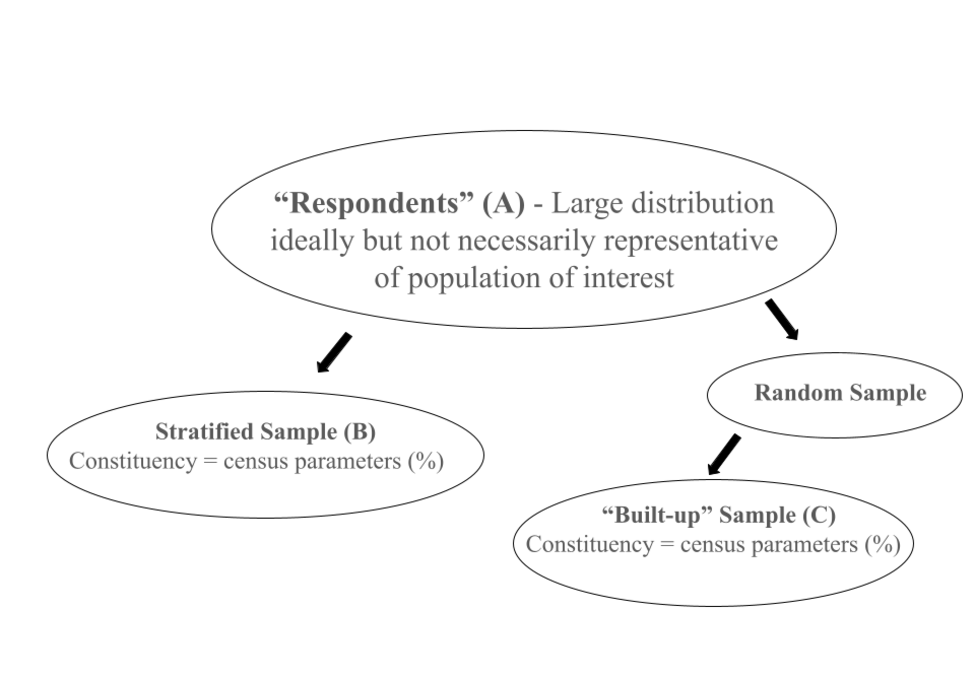
\includegraphics{NormsBuilding_files/figure-latex/schematic-1.pdf}
\caption{\label{fig:schematic}Relationship between Study 1 concepts of population (A), traditional norms (B), and proposed norm building procedure (C).}
\end{figure}

Although seeking representative samples from larger populations comprises the traditional approach to norm-building, alternatives have been sought. Much of this work seems to have peaked (and subsequently perhaps been abandoned) in the 1960's. Lord (1962) may have been one of the first to publicly disseminate an alternative strategy. He describes a procedure first investigated in a 1961 project for the Educational Testing Service (ETS, Lord, 1961) essentially sampling items instead of individuals (e.g., what provides a truer approximation of the population distribution - the entire measure administered to one respondent group or item parcels administered to different respondent groups?). In his first exploration, the ``item sampling'' approach was in fact deemed superior to the more traditional ``respondent sampling'' strategy, with Lord (1961) concluding that such a strategy may be enticing to educational assessment professionals because it is less disruptive (administering smaller item sets requires less time commitment). Plumlee (1964) also administered smaller item subsets to multiple samples of respondants. Both procedures administered smaller item subsets to smaller groups of respondents, and then aggregated from these multiple samples and item sets. The summary finding of each of these studies was that the item subgroup estimates provided better (closer to true normative) estimates than did sub-sample estimates. \textbf{will need to re-read these - current explanation isn't clear} The current investigation revisits these concepts, but with: 1) controlled simulations, and 2) an alternative sample adjustment procedure (the investigations in the 1960's did not attempt weighting). Figure \ref{fig:schematic} communicates our intent: to evaluate the viability of an alternative (C) to the commonly executed (B) norms-development strategy.

\hypertarget{methods}{%
\section{Methods}\label{methods}}

The current exploration utilizes simulations to test the efficacy of the weighting procedure. First, we generate a ``population'' with known subgroup differences along a measured variable representing a scale score from a Psychological inventory (for context, we refer to this as a summary ``engagement'' rating per individual). Next, we \emph{randomly sample} subsets from these populations and build (via post-stratification weighting) representative normative groups. As an index of how the procedure performs, we evaluate the normative distributions against the original population distributions, documenting which distributions (weighted versus unweighted) closer approximates the population engagement value.

\hypertarget{procedure}{%
\subsection{Procedure}\label{procedure}}

\begin{lltable}

\begin{TableNotes}[para]
\normalsize{\textit{Note.} Cell-level constituencies (e.g., percentage white male managers) were not available via census data.}
\end{TableNotes}

\footnotesize{

\begin{longtable}{llllllllll}\noalign{\getlongtablewidth\global\LTcapwidth=\longtablewidth}
\caption{\label{tab:census}}\\
\toprule
Variable & Level & Census
Parameter & Cond 1 & Cond 2 & Cond 3 & Sampling
Frequency & Cond 4 & Cond 5 & Cond 6\\
\midrule
\endfirsthead
\caption*{\normalfont{Table \ref{tab:census} continued}}\\
\toprule
Variable & Level & Census
Parameter & Cond 1 & Cond 2 & Cond 3 & Sampling
Frequency & Cond 4 & Cond 5 & Cond 6\\
\midrule
\endhead
Gender & Male & 53\% &  &  &  &  &  &  & \\
 & Female & 47\% &  &  &  &  &  &  & \\
 &  &  &  &  &  &  &  &  & \\
Ethnicity & White & 78\% & Pos Skew & Normal & Neg Skew & 33\% & Pos Skew & Normal & Neg Skew\\
 & Black & 12\% & Neg Skew & Pos Skew & Normal & 33\% & Neg Skew & Pos Skew & Normal\\
 & Asian or Other & 10\% & Normal & Neg Skew & Pos Skew & 34\% & Normal & Neg Skew & Pos Skew\\
 &  &  &  &  &  &  &  &  & \\
Industry & Management & 40\% &  &  &  &  &  &  & \\
 & Sales & 22\% &  &  &  &  &  &  & \\
 & Service & 17\% &  &  &  &  &  &  & \\
 & Production & 12\% &  &  &  &  &  &  & \\
 & Natural Resources & 9\% &  &  &  &  &  &  & \\
\bottomrule
\addlinespace
\insertTableNotes
\end{longtable}

}

\end{lltable}

Workforce representation was identified via the Bureau of Labor Statistics' Labor Force Statistics from the Current Population Survey (Employed persons by detailed occupation, sex, race, and Hispanic or Latino ethnicity (\href{https://www.bls.gov/cps/cpsaat11.htm}{Table 11}), Statistics, Bureau of Labor, 2018). These are approximately 153,337,000 individuals aged 16 and older. The population percentages were specified at variable margin levels and these values are presented in the ``Census Parameter'' column of Table \ref{tab:census}.

``Populations'' of 10,000 individuals were constructed with ethnic distributions of values specified as normal, positively skewed, or negatively skewed (in three different \emph{across-group} patterns; see Table \ref{tab:census} - this was done to evaluate the impact of different distributional forms within differently sized subgroups). Occupation and gender were then randomly assigned at census parameters (for example, the 1,000 other, 1,200 black, and 7,800 white respondents were randomly assigned gender and occupational characteristics for purposes of multi-strata rating {[}e.g., aka ``raking''{]}). From these 10,000 records, a random or stratified random\footnote{These terms are a bit misleading in the context of the current simulations - all samplings were random, but ``stratified random'' was approximated in conditions 1 through 3 (see Table \ref{tab:census}) whereas differentially stratified was specified in conditions 4 through 6 (where we were interested in evaluating the efficacy of the weighting procedure with known biased {[}in terms of representative constituency{]} samples).} sampling was performed at \emph{n}'s of 100. The samplings were then raked using the \emph{anesrake} (Pasek, 2018) package within \emph{R}. Across the six experimental conditions, populations were specified, sampled from, and raked 10,000 times each (e.g., each of the 60,000 total simulations estimated a different simulated population).

We varied the distributional forms of the three ethic groups, with the distribution of scores (1 to 5) representing negative (1) to positive (5) attitudes. In condition 1, for example, ``Whites'' realized a positively skewed distribution, ``blacks'' were represented with a negatively skewed distribution, and ``asians and others'' exhibited a normally distributed range of attitudes (Figure 2 presents one population simulation as an example of a Condition 1 set of subgroup distributions).

To evaluate the ``quality'' of the random, stratified random, and weighted samples, we collected distributional values at seven different percentile locations: the 5th, 10th, 25th, 50th, 75th, 90th, and 95th percentiles. These values were extracted from: 1) each simulated population, 2) each random or stratified random sampling, and 3) each weighted sample. Our criteria for ``quality'' of normative distribution was discrepancy from the population distributional values at each of the seven percentiles.

\begin{figure}
\centering
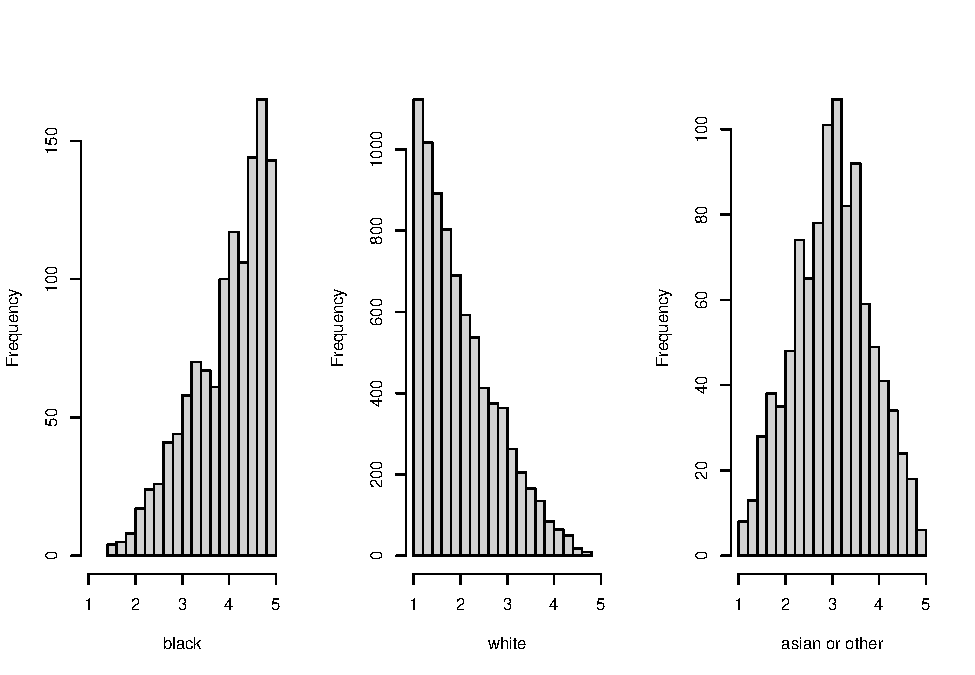
\includegraphics{NormsBuilding_files/figure-latex/Figure2-1.pdf}
\caption{\label{fig:Figure2}Example distributional forms (population specifications Condition 1).}
\end{figure}

The other demographic specifications (occupation and gender) were randomly assigned to the 10,000 ethnic cases (e.g., Table 1 percentages were specified and randomly assigned to cases).

\hypertarget{results}{%
\section{Results}\label{results}}

We present the majority of our results visually in Figures 3 through 8. Because of the ``busy-ness'' of the information within these figures, we present one visual representation of each experimental condition, although every figure conveys the same information: 1) the ``population'' distribution\footnote{These are labeled ``frames'' within Figures 4 through 9 as these simulated distributions could be viewed as representations of either true populations or population frames.} (1st row), 2) discrepancies between population and unweighted sample distribution values at each of the 7 retained percentiles (2nd row), and 3) discrepancies between population and \emph{weighted} sample distribution values (3rd row). The x-axis scales on these discrepancy graphs are intentionally asymmetric toward negative discrepancies because our most extreme outliers were negative (although not possible to visually see within the histograms). Negative values indicate a ``larger'' population than sample value. Conditions 1 through 3 demonstrate that, regardless of distributional form across the small or large constituent groups, if sampling can be reasonably characterized as stratified (e.g., if the sample has representative constituencies), there is no need or indeed added value in weighting the sample (this is admittedly not an exceedingly earth-shattering finding, but if the sample already approximates the population, there is in fact no need for weighting).

\begin{figure}
\centering
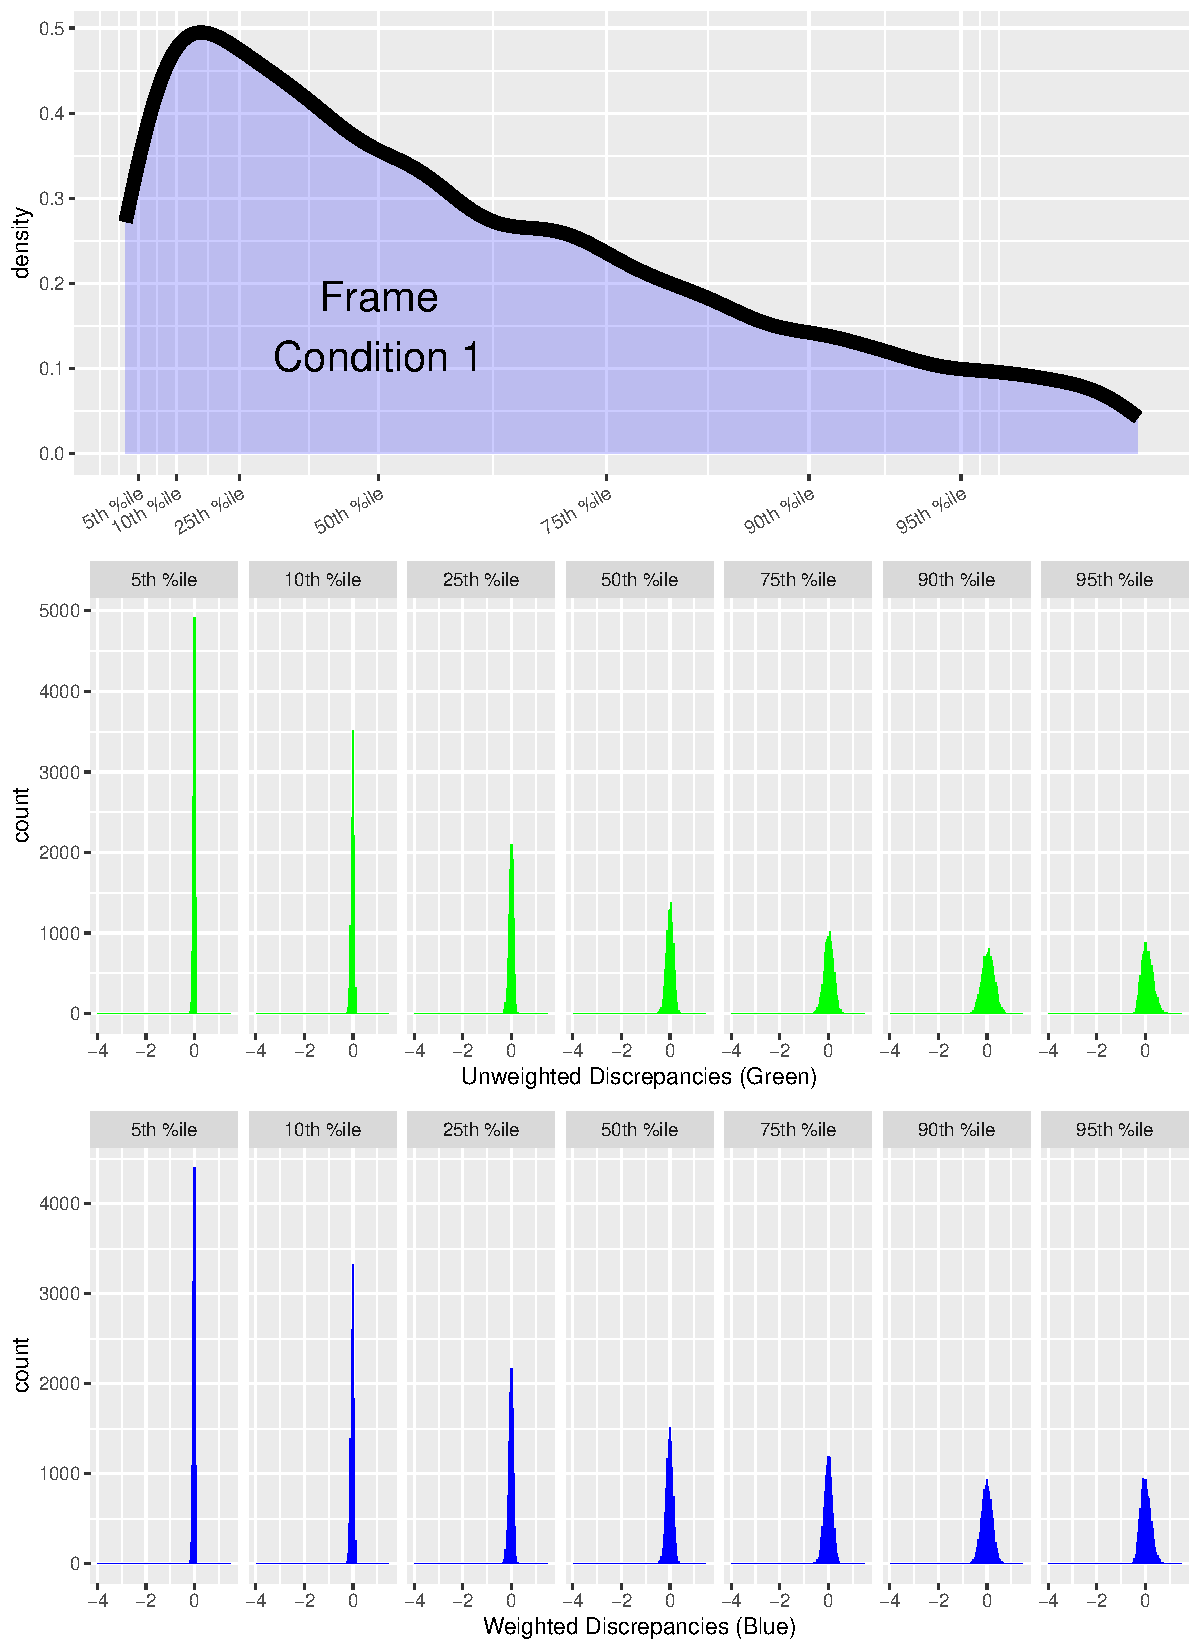
\includegraphics{NormsBuilding_files/figure-latex/Figure3-1.pdf}
\caption{\label{fig:Figure3}Population percentile locations with unweighted (approximately stratified), and weighted discrepancy distributions (Condition 1).}
\end{figure}

\begin{figure}
\centering
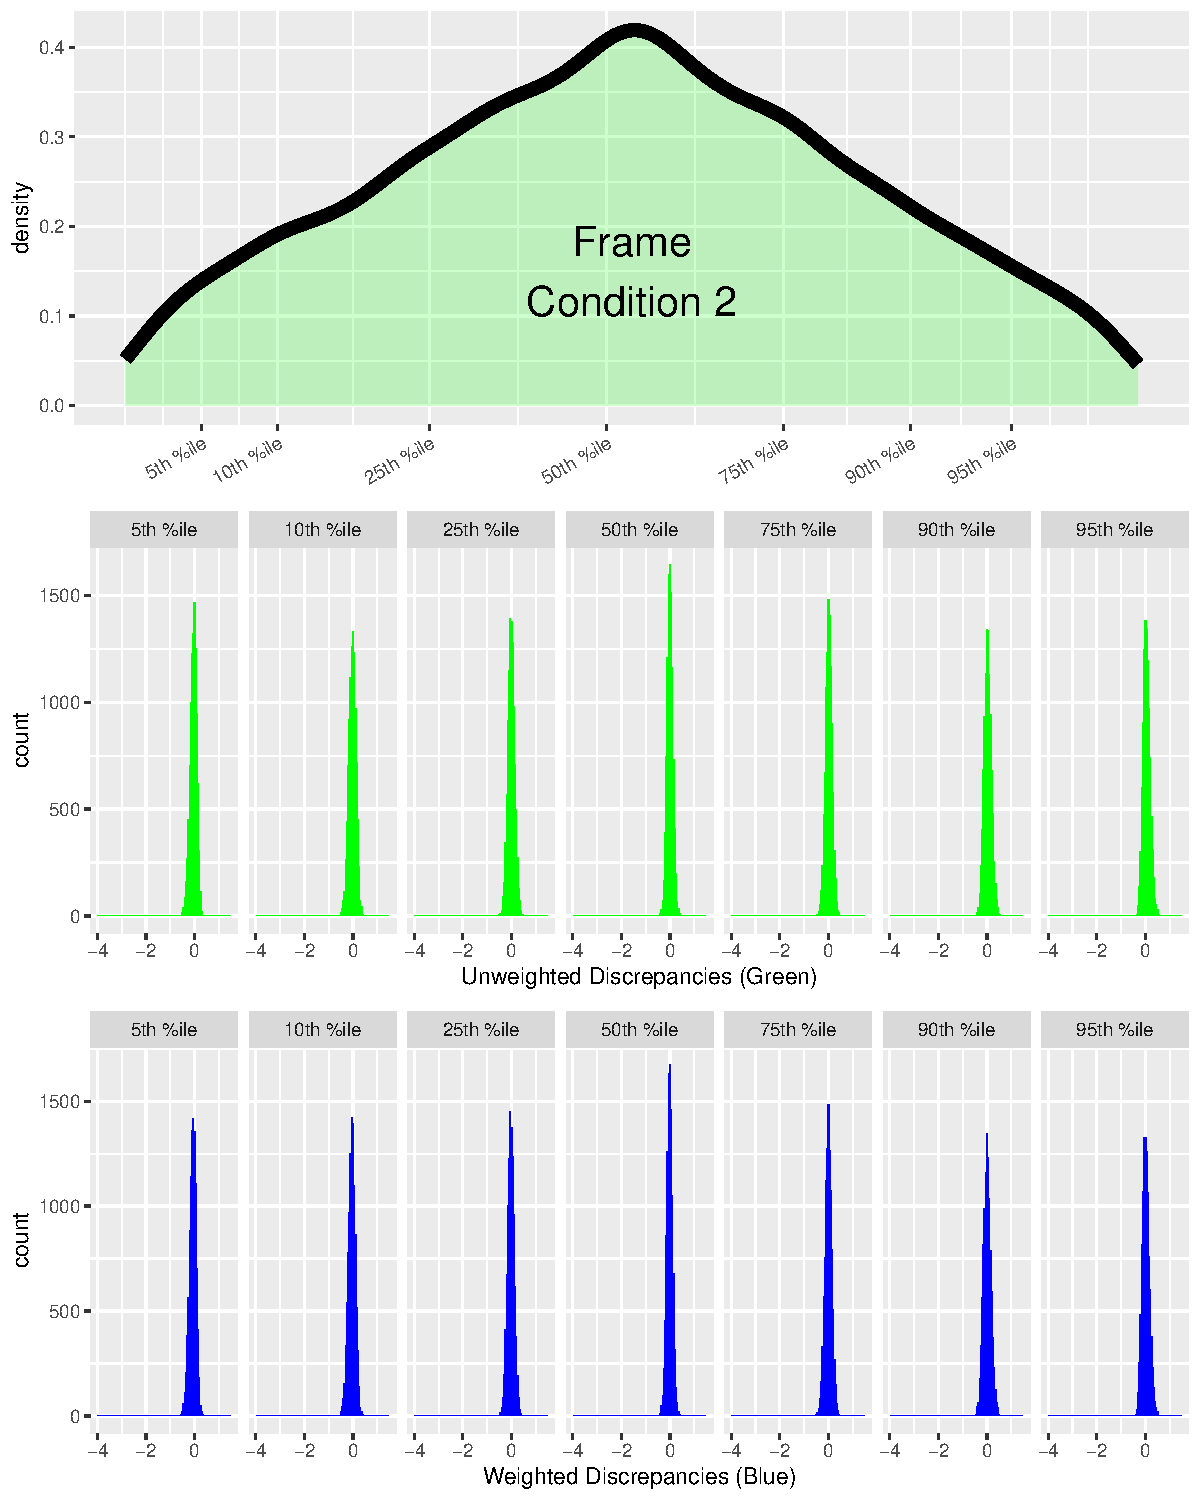
\includegraphics{NormsBuilding_files/figure-latex/Figure4-1.pdf}
\caption{\label{fig:Figure4}Population percentile locations with unweighted (approximately stratified), and weighted discrepancy distributions (Condition 2).}
\end{figure}

\begin{figure}
\centering
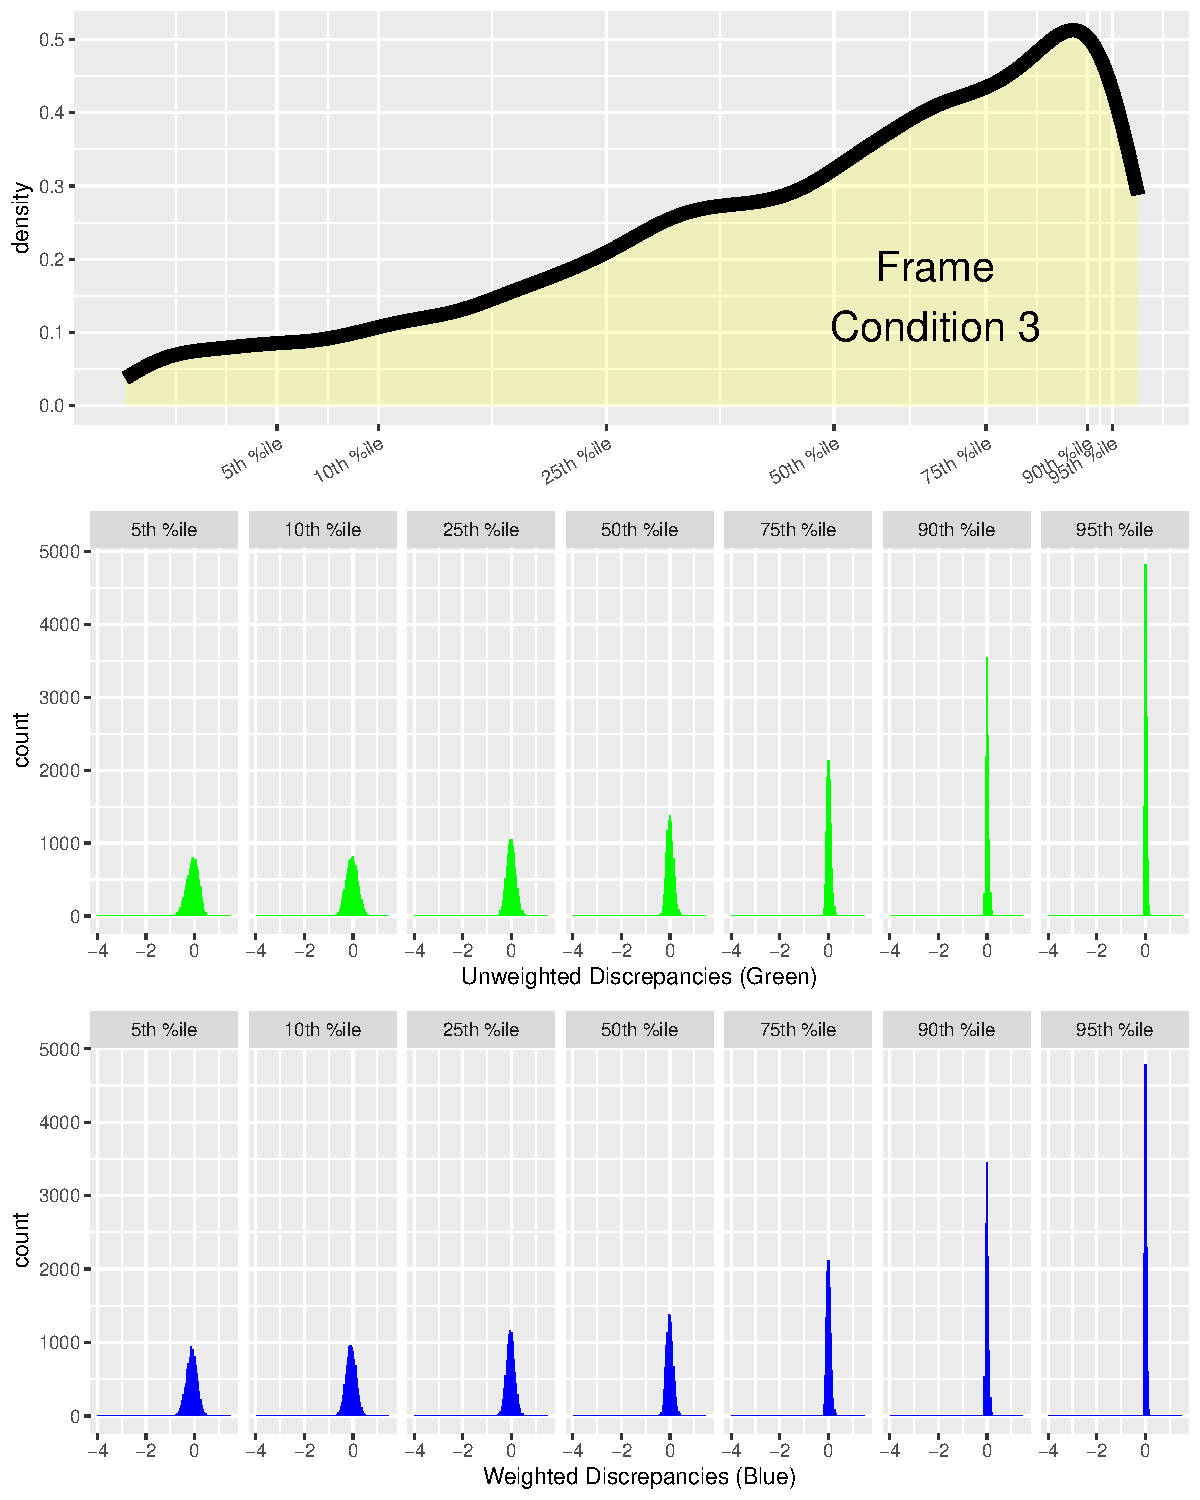
\includegraphics{NormsBuilding_files/figure-latex/Figure5-1.pdf}
\caption{\label{fig:Figure5}Population percentile locations with unweighted (approximately stratified), and weighted discrepancy distributions (Condition 3).}
\end{figure}

\begin{figure}
\centering
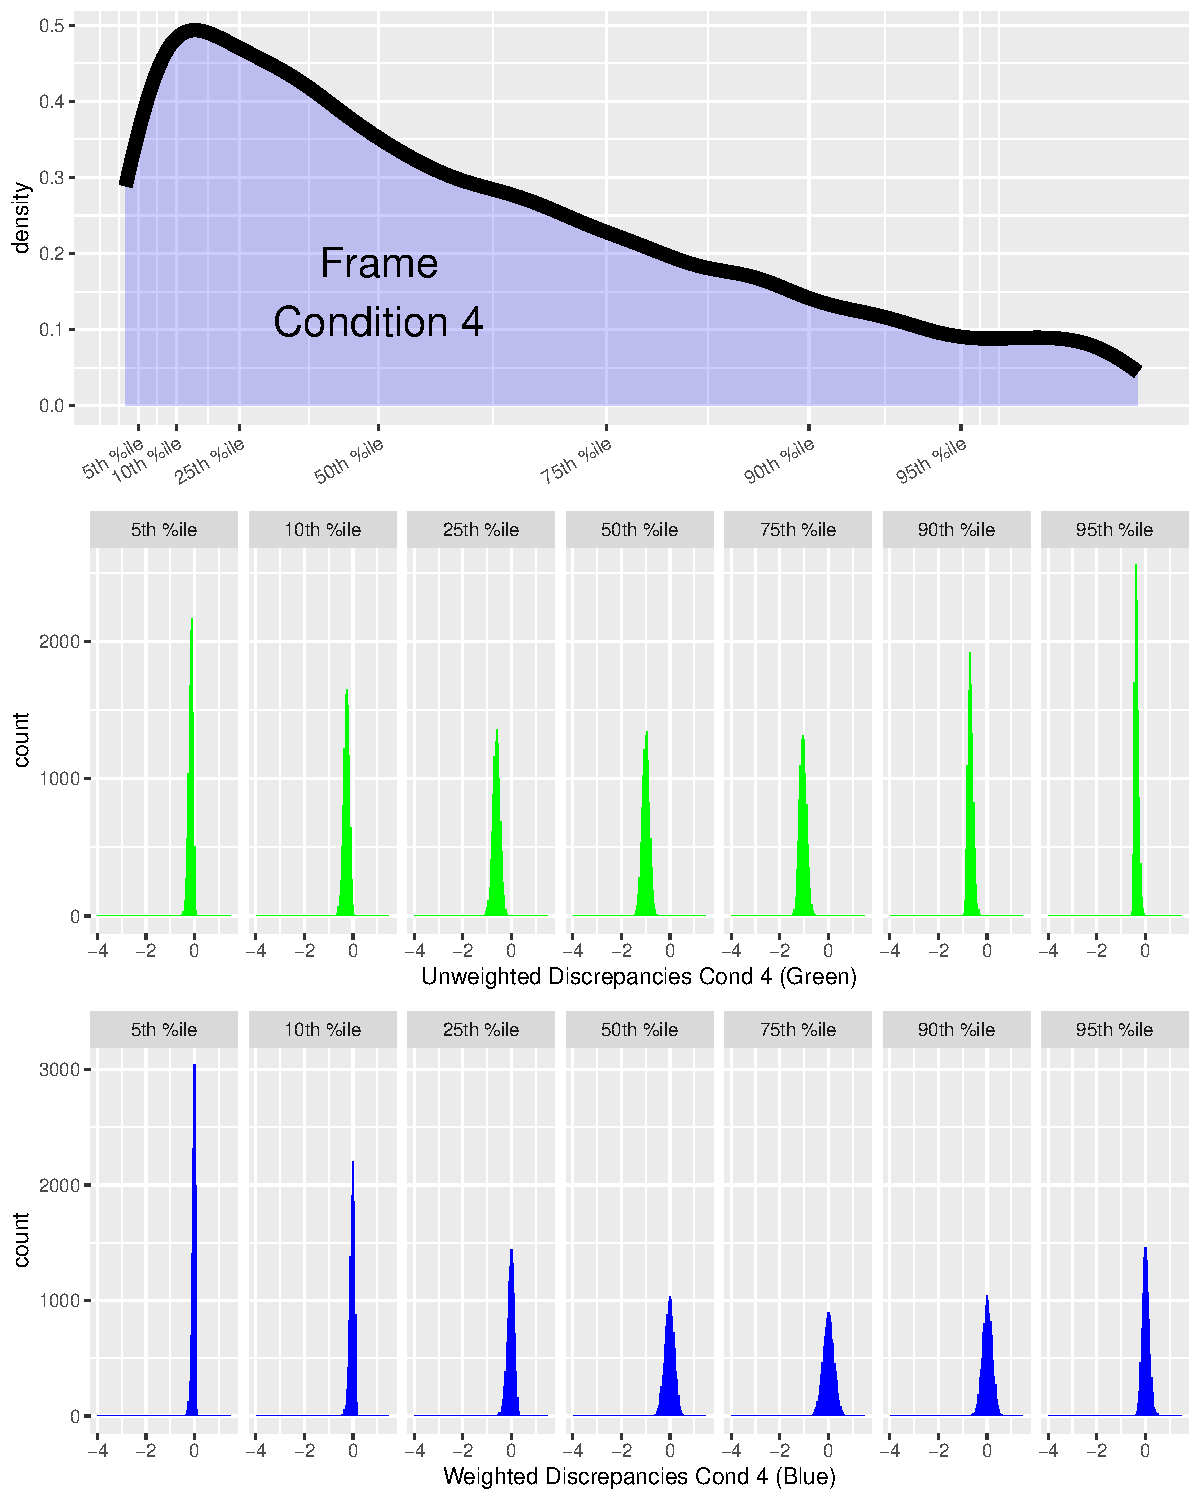
\includegraphics{NormsBuilding_files/figure-latex/Figure6-1.pdf}
\caption{\label{fig:Figure6}Population percentile locations with unweighted (disproportionate), and weighted discrepancy distributions (Condition 4).}
\end{figure}

\begin{figure}
\centering
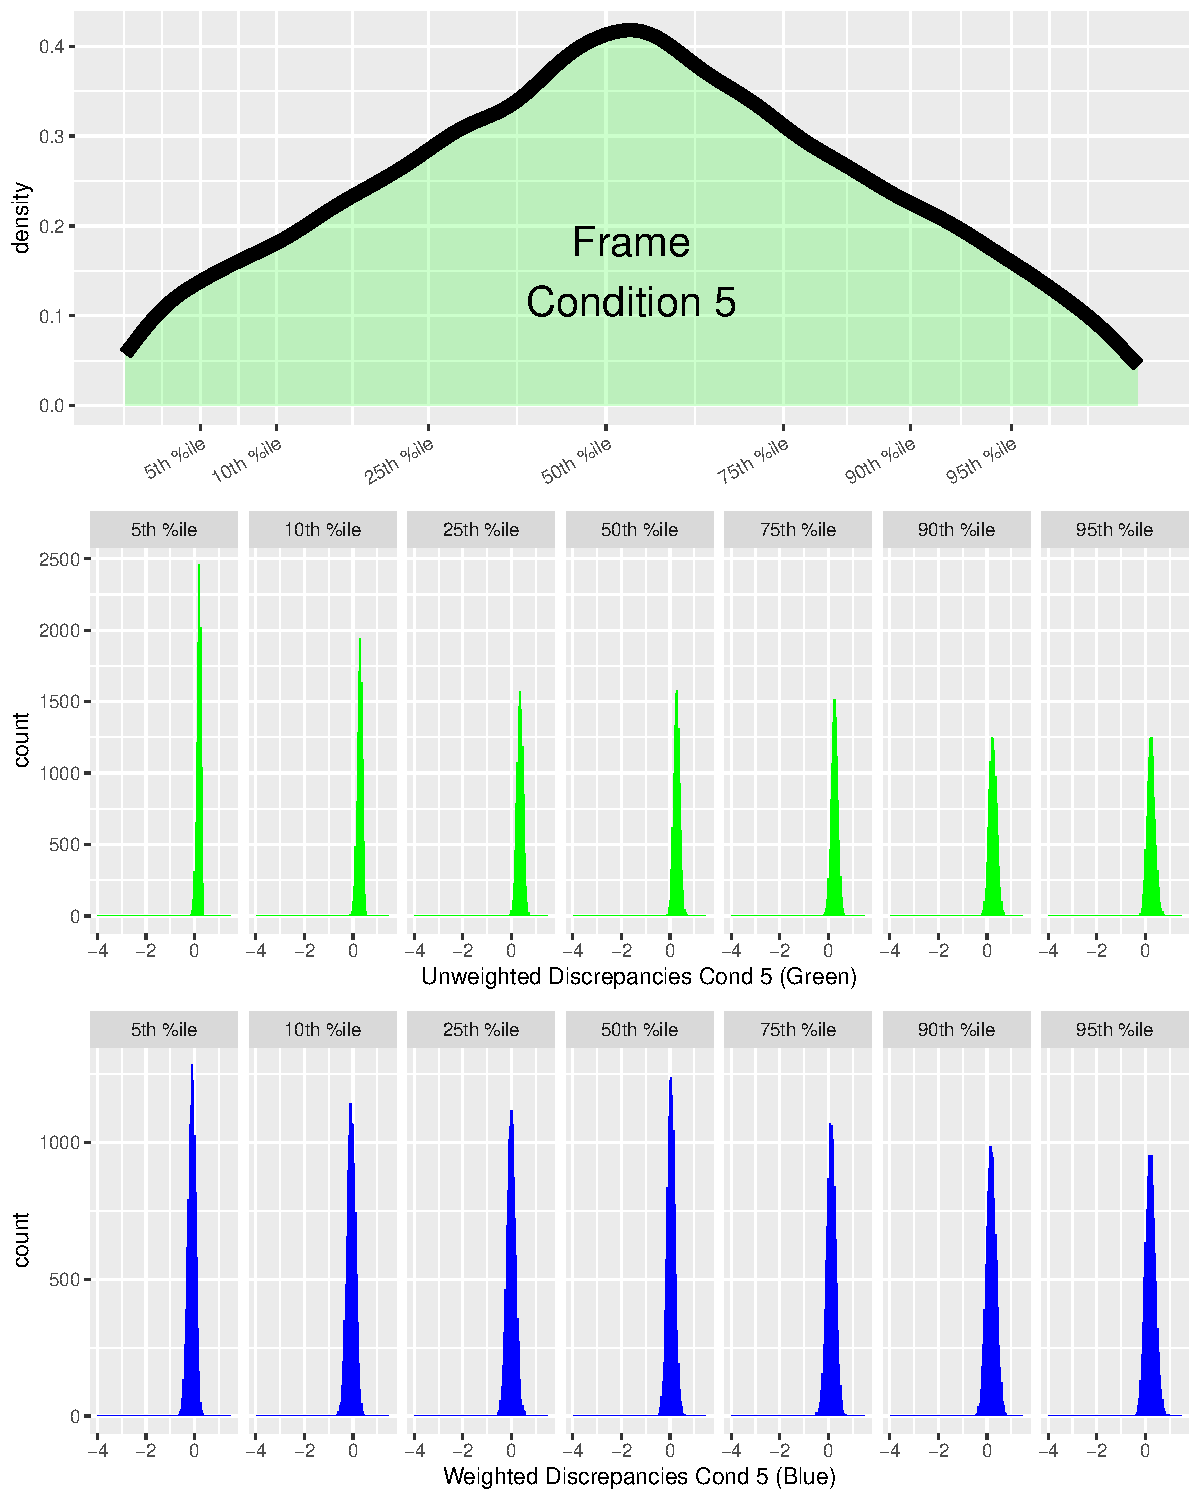
\includegraphics{NormsBuilding_files/figure-latex/Figure7-1.pdf}
\caption{\label{fig:Figure7}Population percentile locations with unweighted (disproportionate), and weighted discrepancy distributions (Condition 5).}
\end{figure}

\begin{figure}
\centering
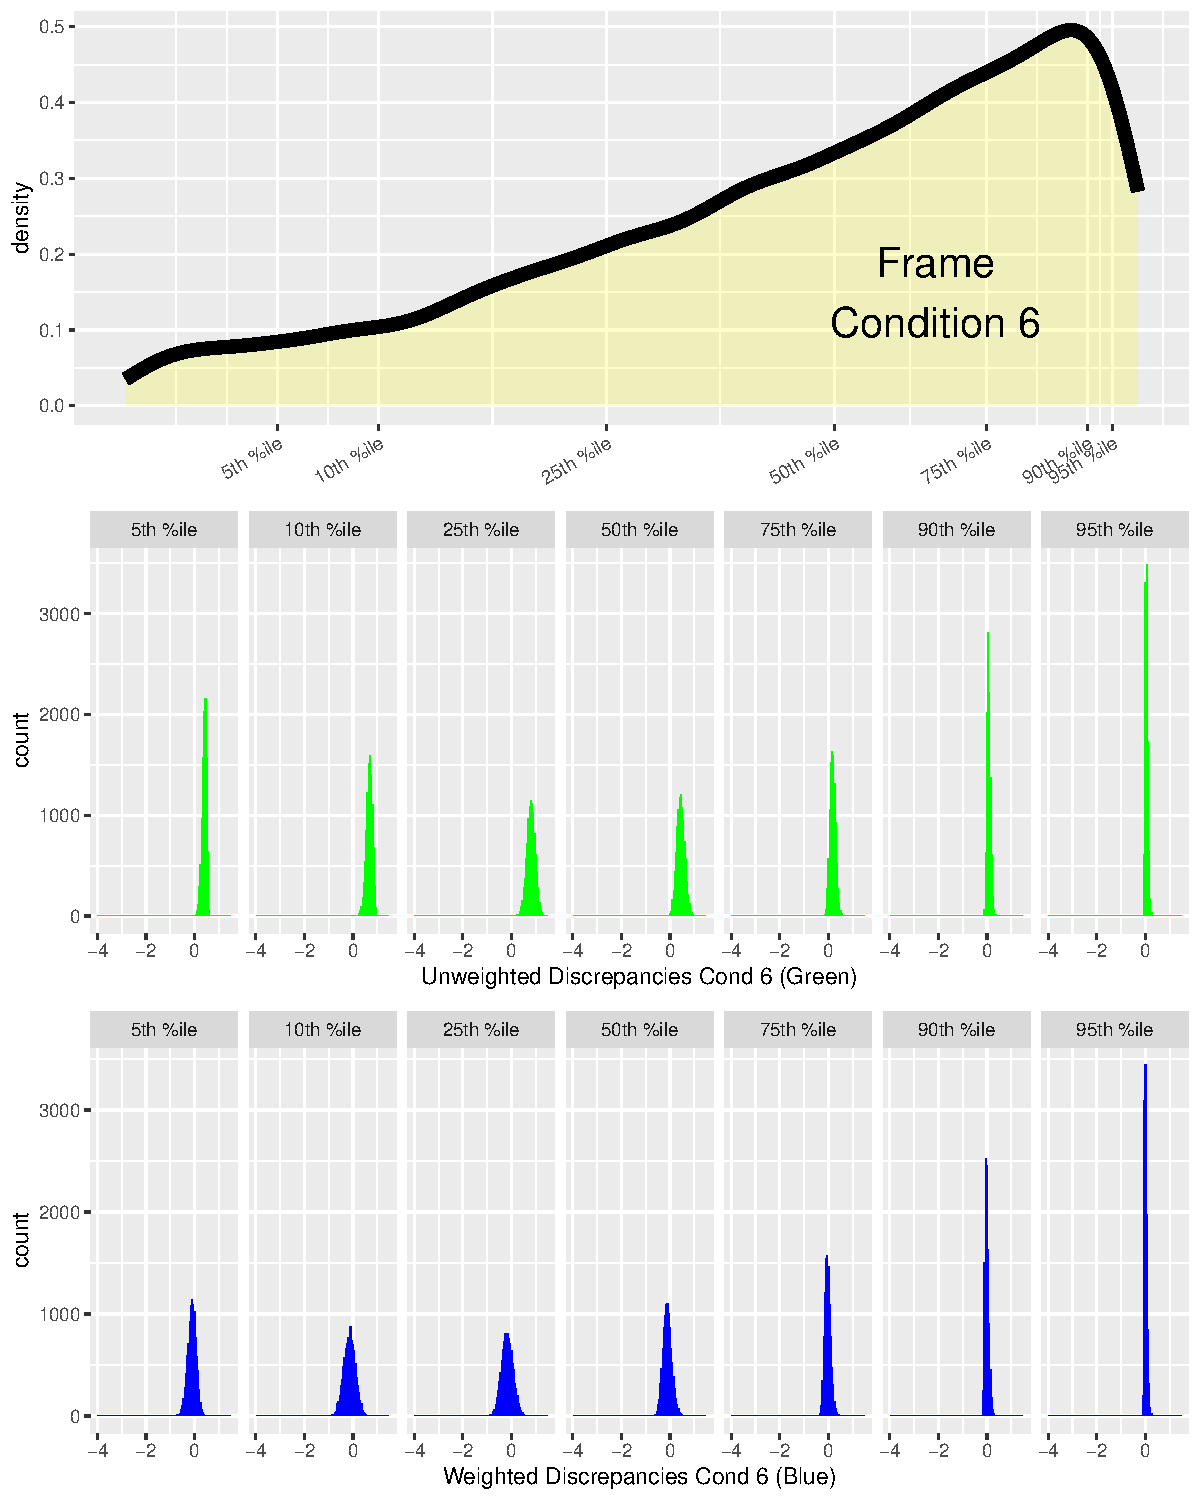
\includegraphics{NormsBuilding_files/figure-latex/Figure8-1.pdf}
\caption{\label{fig:Figure8}Population percentile locations with unweighted (disproportionate), and weighted discrepancy distributions (Condition 6).}
\end{figure}

Conditions 4 through 6, however (Figures 6 through 8) demonstrate that weighted normative distributions do far exceed the quality of randomly sampled distributions if those random samplings result in subgroup proportional inconsistencies (e.g., not representative constituency). The narrow nature of these distributions of discrepancies (regardless of whether the distribution is weighted or unweighted) shows that the samplings result in largely similar values across the 10,000 simulations. The \emph{location} of the distributions, however, highlights the advantage of weighting: the unweighted samples deviate from centering on a value of zero (zero indicates a population-sample match at the percentile of focus). Discrepancy distributions centering on non-zero values represent \emph{bias} in the normative values. In all three conditions where bias was present (at at least one percentile location), performing the weighting corrected this bias.

\hypertarget{discussion}{%
\section{Discussion}\label{discussion}}

Post-stratification weighting does appear to hold some promise as a norms-building strategy. Particularly in situations where frames (or even merely larger samples) are not proportionally representative of populations, the weighting procedure effectively reproduces the output of stratified sampling: producing a proportionally representative sample distribution. We attempted to introduce large constituent group differences in distributional forms (within the ``populations'') as a challenge to the weighting procedure, but, as long as strata are properly identified (along which value distributions may vary), the resulting weighted distribution does do a very good job at representing the population distribution (much better than does the unweighted normative distribution). Future investigations should introduce additional discrepancies (both distributional as well as subgroup proportional) to further test the boundaries of the procedure. Attempts to ``construct'' representative norms with real-world data are also warrented.

Scale development papers should devote some attention to their norms creation - speculate that much of this is located in technical reports, but those are not as commonly available to researchers.

\newpage

\hypertarget{references}{%
\section{References}\label{references}}

\begingroup
\setlength{\parindent}{-0.5in}
\setlength{\leftskip}{0.5in}

\hypertarget{refs}{}
\begin{CSLReferences}{1}{0}
\leavevmode\vadjust pre{\hypertarget{ref-gillespie2016normative}{}}%
Gillespie, M. A., Balzer, W. K., Brodke, M. H., Garza, M., Gerbec, E. N., Gillespie, J. Z., Gopalkrishnan, P., Lengyel, J. S., Sliter, K. A., Sliter, M. T., et al. (2016). Normative measurement of job satisfaction in the US. \emph{Journal of Managerial Psychology}, \emph{31}(2), 516--536.

\leavevmode\vadjust pre{\hypertarget{ref-hawkins2002norms}{}}%
Hawkins, K. A., \& Bender, S. (2002). Norms and the relationship of boston naming test performance to vocabulary and education: A review. \emph{Aphasiology}, \emph{16}(12), 1143--1153.

\leavevmode\vadjust pre{\hypertarget{ref-holt_stanford_1993}{}}%
Holt, J. A. (1993). Stanford achievement test---8th edition: Reading comprehension subgroup results. \emph{American Annals of the Deaf}, \emph{138}(2), 172--175.

\leavevmode\vadjust pre{\hypertarget{ref-kinnear_new_2002}{}}%
Kinnear, P. R., \& Sahraie, A. (2002). New farnsworth-munsell 100 hue test norms of normal observers for each year of age 5--22 and for age decades 30--70. \emph{The British Journal of Ophthalmology}, \emph{86}(12), 1408--1411. \url{https://www.ncbi.nlm.nih.gov/pmc/articles/PMC1771429/}

\leavevmode\vadjust pre{\hypertarget{ref-kulas_post-stratification_2018}{}}%
Kulas, J. T., Robinson, D. H., Smith, J. A., \& Kellar, D. Z. (2018). Post-stratification weighting in organizational surveys: A cross-disciplinary tutorial. \emph{Human Resource Management}.

\leavevmode\vadjust pre{\hypertarget{ref-lord1961estimating}{}}%
Lord, F. M. (1961). Estimating norms by item sampling. \emph{ETS Research Bulletin Series}, \emph{1961}(1), i--13.

\leavevmode\vadjust pre{\hypertarget{ref-lord_estimating_1962}{}}%
Lord, F. M. (1962). Estimating norms by item-sampling. \emph{Educational and Psychological Measurement}, \emph{22}(2), 259--267. \url{https://doi.org/10.1177/001316446202200202}

\leavevmode\vadjust pre{\hypertarget{ref-R-anesrake}{}}%
Pasek, J. (2018). \emph{Anesrake: ANES raking implementation}. \url{https://CRAN.R-project.org/package=anesrake}

\leavevmode\vadjust pre{\hypertarget{ref-plumlee1964estimating}{}}%
Plumlee, L. B. (1964). Estimating means and standard deviations from partial data---an empirical check on lord's item sampling technique. \emph{Educational and Psychological Measurement}, \emph{24}(3), 623--630.

\leavevmode\vadjust pre{\hypertarget{ref-shl2011}{}}%
SHL Group Ltd. (2011). \emph{OPQ32r norm update technical documentation} {[}Technical Report{]}. SHL Group Ltd.

\leavevmode\vadjust pre{\hypertarget{ref-statistics_cps_2018}{}}%
Statistics, Bureau of Labor. (2018). \emph{{CPS} tables}. \url{https://www.bls.gov/cps/tables.htm}

\leavevmode\vadjust pre{\hypertarget{ref-tombaugh_60-item_1997}{}}%
Tombaugh, T. N., \& Hubiey, A. M. (1997). The 60-item boston naming test: Norms for cognitively intact adults aged 25 to 88 years. \emph{Journal of Clinical and Experimental Neuropsychology}, \emph{19}(6), 922--932.

\leavevmode\vadjust pre{\hypertarget{ref-yang_nonresponse_2017}{}}%
Yang, Y., Kulas, J. T., \& Robinson, D. R. (2017, April). \emph{Nonresponse and sample weighting in organizational surveying}. Society for industrial and organizational psychology.

\leavevmode\vadjust pre{\hypertarget{ref-zec_normative_2007}{}}%
Zec, R. F., Burkett, N. R., Markwell, S. J., \& Larsen, D. L. (2007). Normative data stratified for age, education, and gender on the boston naming test. \emph{The Clinical Neuropsychologist}, \emph{21}(4), 617--637. \url{https://doi.org/10.1080/13854040701339356}

\end{CSLReferences}

\endgroup


\end{document}
